\documentclass[tikz,border=12pt]{standalone}
\usepackage[utf8]{inputenc}
\usepackage{tikz}
\usetikzlibrary{shapes,arrows.meta,positioning,calc}

\definecolor{ScoutGreen}{HTML}{005432}
\definecolor{ScoutNavy}{HTML}{002855}
\definecolor{ScoutBlue}{HTML}{006EB6}
\definecolor{ScoutRed}{HTML}{A31920}
\definecolor{ScoutAmber}{HTML}{D97706}
\definecolor{BorderGray}{HTML}{CBD5E1}

\begin{document}
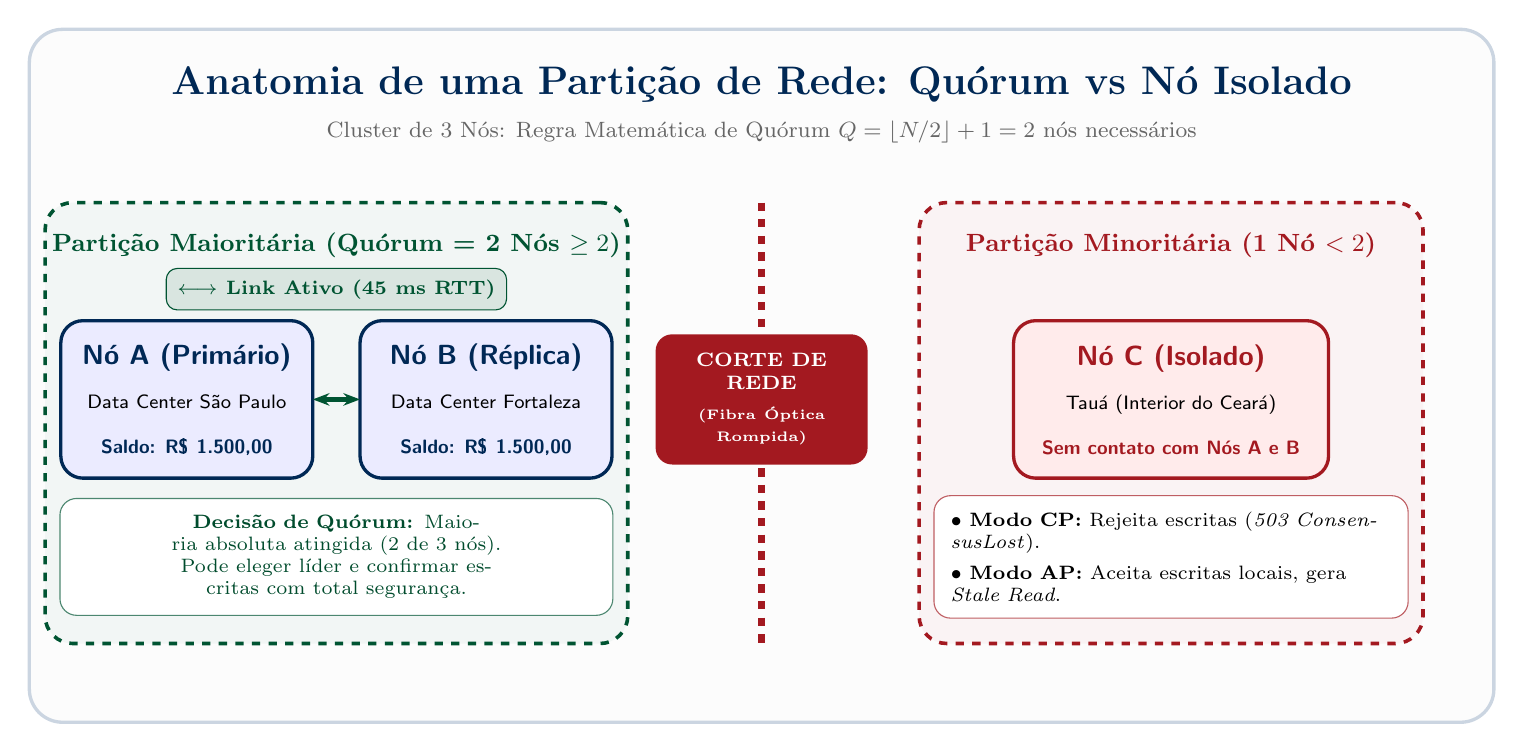
\begin{tikzpicture}[
    font=\sffamily,
    no/.style={draw=BorderGray, rounded corners=8pt, fill=white, line width=1.2pt, align=center, inner sep=6pt}
]

  % Painel Fundo Geral
  \node[draw=BorderGray, rounded corners=12pt, fill=gray!2, line width=1.2pt, minimum width=18.6cm, minimum height=8.8cm] (bg) at (0, 0) {};
  
  \node[font=\bfseries\Large, text=ScoutNavy] at (0, 3.7) {Anatomia de uma Partição de Rede: Quórum vs Nó Isolado};
  \node[font=\footnotesize, text=gray!80!black] at (0, 3.1) {Cluster de 3 Nós: Regra Matemática de Quórum $Q = \lfloor N/2 \rfloor + 1 = 2$ nós necessários};

  % =========================================================================
  % ÁREA DA MAIORIA (QUÓRUM ATINGIDO) - LADO ESQUERDO
  % =========================================================================
  \node[draw=ScoutGreen, dashed, rounded corners=10pt, fill=ScoutGreen!5, line width=1.3pt, minimum width=7.4cm, minimum height=5.6cm] (area_maioria) at (-5.4, -0.6) {};
  \node[font=\small\bfseries, text=ScoutGreen, anchor=north] at (area_maioria.north) [yshift=-8pt] {Partição Maioritária (Quórum = 2 Nós $\ge 2$)};

  % Nó A
  \node[no, draw=ScoutNavy, fill=blue!8, minimum width=3.2cm, minimum height=2.0cm] (no_a) at (-7.3, -0.3) {
    \textbf{\color{ScoutNavy}\normalsize Nó A (Primário)}\\[4pt]
    {\scriptsize Data Center São Paulo}\\[4pt]
    {\scriptsize \color{ScoutNavy}\textbf{Saldo: R\$ 1.500,00}}
  };

  % Nó B
  \node[no, draw=ScoutNavy, fill=blue!8, minimum width=3.2cm, minimum height=2.0cm] (no_b) at (-3.5, -0.3) {
    \textbf{\color{ScoutNavy}\normalsize Nó B (Réplica)}\\[4pt]
    {\scriptsize Data Center Fortaleza}\\[4pt]
    {\scriptsize \color{ScoutNavy}\textbf{Saldo: R\$ 1.500,00}}
  };

  % Link ativo entre A e B
  \draw[{Stealth[length=6pt]}-{Stealth[length=6pt]}, line width=2pt, color=ScoutGreen] (-5.7, -0.3) -- (-5.1, -0.3);
  \node[fill=ScoutGreen!15, draw=ScoutGreen, rounded corners=4pt, font=\scriptsize\bfseries, text=ScoutGreen, inner sep=4pt] at (-5.4, 1.1) {
    $\longleftrightarrow$ Link Ativo (45 ms RTT)
  };

  % Decisão do Quórum
  \node[draw=ScoutGreen!70, fill=white, rounded corners=6pt, font=\scriptsize, text=ScoutGreen!90!black, align=center, text width=6.6cm, inner sep=6pt] at (-5.4, -2.3) {
    \textbf{Decisão de Quórum:} Maioria absoluta atingida (2 de 3 nós).\\
    Pode eleger líder e confirmar escritas com total segurança.
  };

  % =========================================================================
  % LINHA DE CORTE DE REDE (CORREDOR CENTRAL DEDICADO - LIVRE DE COLISÕES)
  % =========================================================================
  \draw[dashed, line width=2.5pt, color=ScoutRed] (0, 2.2) -- (0, -3.4);
  \node[fill=ScoutRed, text=white, rounded corners=6pt, font=\bfseries\scriptsize, align=center, inner sep=7pt, text width=2.2cm] at (0, -0.3) {
    \textbf{CORTE DE\\REDE}\\[3pt]
    {\tiny (Fibra Óptica Rompida)}
  };

  % =========================================================================
  % ÁREA DA MINORIA (NÓ ISOLADO) - LADO DIREITO
  % =========================================================================
  \node[draw=ScoutRed, dashed, rounded corners=10pt, fill=ScoutRed!5, line width=1.3pt, minimum width=6.4cm, minimum height=5.6cm] (area_minoria) at (5.2, -0.6) {};
  \node[font=\small\bfseries, text=ScoutRed, anchor=north] at (area_minoria.north) [yshift=-8pt] {Partição Minoritária (1 Nó $< 2$)};

  % Nó C
  \node[no, draw=ScoutRed, fill=red!8, minimum width=4.0cm, minimum height=2.0cm] (no_c) at (5.2, -0.3) {
    \textbf{\color{ScoutRed}\normalsize Nó C (Isolado)}\\[4pt]
    {\scriptsize Tauá (Interior do Ceará)}\\[4pt]
    {\scriptsize \color{ScoutRed}\textbf{Sem contato com Nós A e B}}
  };

  % Comportamento sob CP vs AP
  \node[draw=ScoutRed!70, fill=white, rounded corners=6pt, font=\scriptsize, align=left, text width=5.6cm, inner sep=6pt] at (5.2, -2.3) {
    $\bullet$ \textbf{Modo CP:} Rejeita escritas (\textit{503 ConsensusLost}).\\[3pt]
    $\bullet$ \textbf{Modo AP:} Aceita escritas locais, gera \textit{Stale Read}.
  };

\end{tikzpicture}
\end{document}
